\documentclass[12pt]{report}
\usepackage{graphicx} %LaTeX package to import graphics
\usepackage[top=2cm, bottom=2cm, left=1.5cm, right=1.5cm]{geometry}

\graphicspath{{images/}} %configuring the graphicx package
 
\title{RayTracing in eucledian space}
\author{Blaž Pirc, Matej Mlakar, Aleks Kožar\thanks{Funded by the Overleaf team.}}
\date{April 2025}

\begin{document}
\maketitle

\tableofcontents

\renewcommand{\abstractname}{Introduction}
\begin{abstract}
    We made Ray-Tracing in Euclidean space, which simulates how light bounces around, brightens objects, causes shades\dots .
    For simulation we implemented a \emph{camera}, which was an array of vectors, \emph{light sources} as points and a variety of \emph{objects} as 3-dimensional functions, such as a sphere, elipsoid, torus and some periodic functions.
    There are 3 material types of objects we implemented, which are \emph{glass, mirror and basic} material, where each object reacts differently to light.
    For the \emph{light source} we implemented so that there are more of them, their power of brightness fades over the distance travelled and each light source emits can emit any color white,green,blue\dots.
\end{abstract}
\chapter{Ray-Tracing implementation}
\section{Drawing the rays}
    The first step of building a ray tracer is to make \emph{rays}, that shoot out from a position in space called \emph{camera}.
    We position the camera at [0, 0, 0] and from there shoot out our rays. The number of rays depends on the specified resolution. 
    They are uniformly spaced out according to the predetermined \emph{FOV} and \emph{aspect ratio} that can also be adjusted. 
    To determine the angle at which each ray shoots out the camera we use simple trigonometry. 
    The result of this is a \emph{2D image}, where each ray represents a single pixel in the picture. 
    \begin{figure}[h]
        \centering
        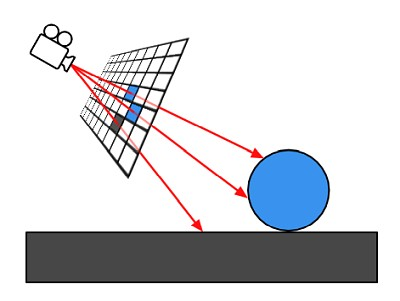
\includegraphics[height=10\baselineskip,keepaspectratio]{camera}  
        \caption{An image visualizing an idea of drawing the rays}
    \end{figure}
    Each ray has various objects on its path. To calculate which objects it collides with, we have a for-loop, that iteratively increases the size of the ray by multiplying it with a \emph{scalar value}.
    For each ray we calculate the first \emph{intersection} with all our objects in scene. This initial intersection is just a rough estimate of the real intersection.
    To calculate a more precise intersection we use \emph{newton’s method}. But firstly we had to parametrize the function and transform it from searching the approximate value in 3d space to determining the value in 1d space. 
    If this method fails to give us a precise enough point after maximum number of iteration, we use a simple bisection to find a zero between two points. Bisection proved itself to be a more reliable, yet slower method. 
    Its simplicity was very welcomed when trying to debug code and fix various issues.
    After all the intersections are determined, we pick out the closest one to our camera and process it further.

\section{Coloring pixels}
    Now that we have a point in space, we need to color it. We do that by calculating the angle between the normal in that point on the object and the light source.
    We get the normal vector by inserting intersection point in the object’s gradient function. The smaller the angle between the normal vector and the light source, the brighter the color. 
    If the angle is larger than 90 degrees we just color it black, because it doesn’t receive any light. The dot product between previously mentioned vectors gives out a scaler value between 0 and 1. 
    We multiply that value by the color of our light source to get a more realistic light contribution. We also decided that we want our light source to lose its luminance with distance. 
    In order to do that we need to calculate light’s power value, which is essentially calculated by formula:
    
    \[ 
        \frac{lightPower}{{dist(object, light)}^{1.2}}
    \]
    
    By changing the power of the formula, we can modify the curve at which light source looses its luminance. To get the final color we multiply this power factor with the previously calculated light contribution.
    We also decided to implement option for multiple lightsources, which means we had to compute everything I’ve mentioned before for every light source and sum it up together 

\end{document}